\chapter{Models}
\label{cha:models}

Single-Image Super Resolution refers to the process of enhancing the size of small images while striving to minimize the reduction in quality or the loss of detail. Alternatively, it involves the task of reconstructing High Resolution (HR) images by utilizing the abundant information present in Low Resolution (LR) images, which lack finer details.

In other words, Image Super Resolution is about taking images that are of lower quality or resolution and applying techniques to enlarge them without significantly sacrificing their overall quality. This can be particularly useful in scenarios where higher resolution images are required for tasks like printing, displaying on high-resolution screens, or analyzing intricate details in images. The goal is to generate visually appealing results that closely resemble the appearance of true high-resolution images or at least contain improved details compared to the original low-resolution versions.

Neural networks are the perfect tool for this kind of task, from a set of images they are capable of capturing a lot of low-level image statistics and creating powerful high-order models able to deal with a very large degradation space.

The models have been chosen taking into account different characteristics. ESRGAN and Real-ESRGAN are two of the most popular models when it comes to Super Resolution, they share a similar structure and both use a GAN (Generative Adversal Network) architecture, on the other hand, HAT-L and SwinIR are transformer-based models that take a new approach to vision tasks.

All models score highly in the ranking proposed by paperswithcode\cite{pwcode}, which provides a leveled field for comparing the latest models of the most common benchmark datasets.

The four models are implemented in the PyTorch-based open-source image and video restoration toolbox BasicSR (Basic Super Restoration). On top of offering the various models for SR it's equipped with useful logging capabilities and metrics for evaluation.


\section{ESRGAN}
\label{subsec:esrgan}

ESRGAN is based on the SRGAN\cite{ledig2017photorealistic} model. SRGAN, is a generative adversarial network (GAN) for image super-resolution (SR). The SRGAN model uses a perceptual loss function that consists of an adversarial loss and a content loss. The adversarial loss pushes the solution to the natural image manifold using a discriminator network that is trained to differentiate between the super-resolved images and original photo-realistic images. In addition, the authors use a content loss motivated by perceptual similarity instead of similarity in pixel space. The actual networks consist mainly of residual blocks for feature extraction. The perceptual loss function is written as a weighted sum of a VGG content loss and an adversarial loss component. SRGAN is capable of inferring photo-realistic natural images for 4x upscaling factors and is the first framework to achieve this.

\begin{figure}[H]
  \centering
  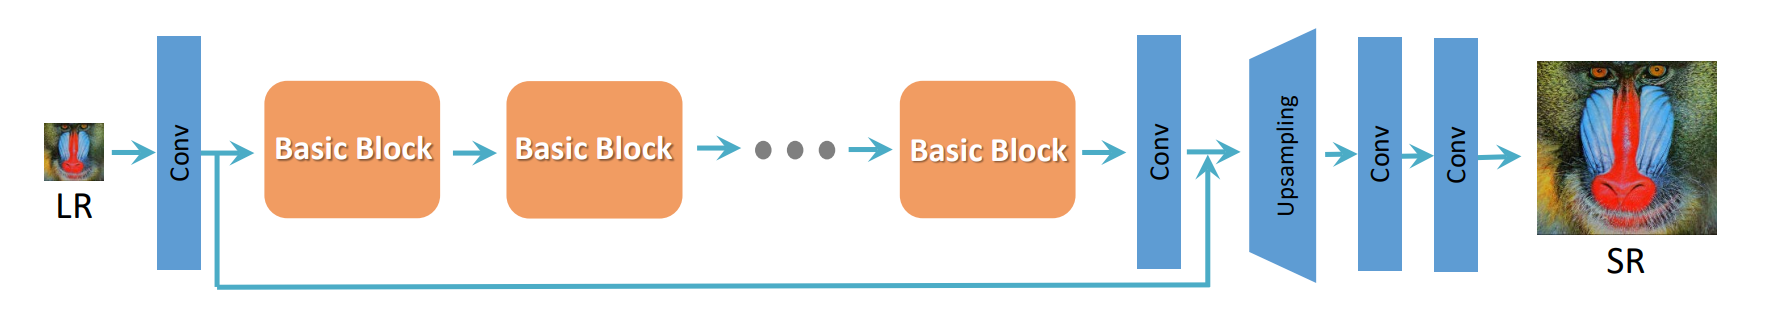
\includegraphics[scale=0.25]{figures/SRResNet.png}
  \caption{The basic architecture of SRResNet.\cite{wang2018esrgan}}
  \label{img:SRResNet}
\end{figure}

ESRGAN stands for Enhanced SRGAN and introduces some major improvements to the framework. The core structure of the network employs an SRResNet architecture (Figure \ref{img:SRResNet}) with two notable differences: the lack of batch normalization and a new structure that replaces the original basic block with the proposed Residual-in-Residual Dense Block (RRDB), which combines multi-level residual network and dense
connections as depicted in Figure \ref{img:RRDB}

\begin{figure}[H]
  \centering
  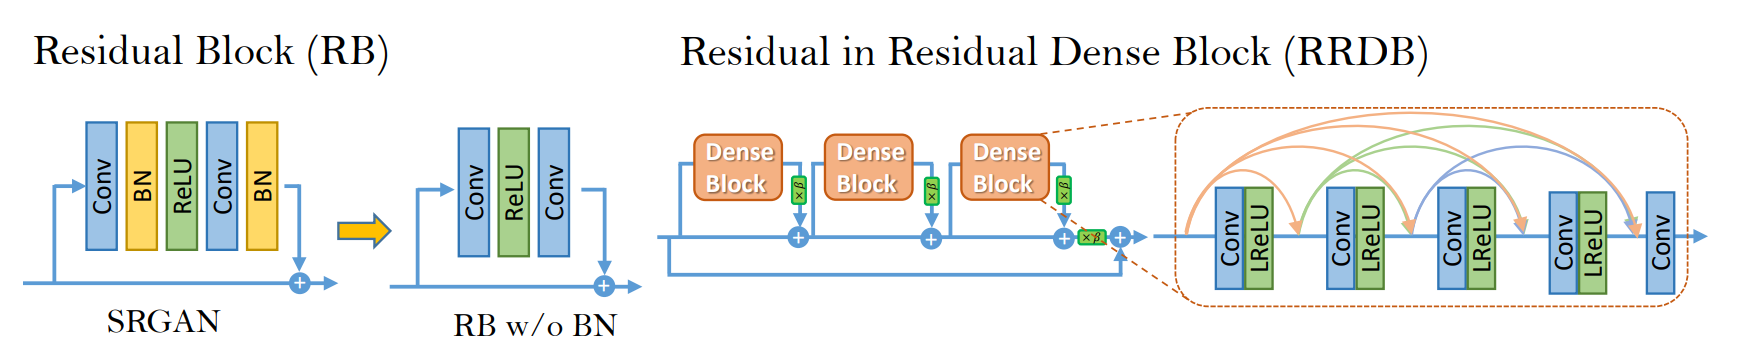
\includegraphics[scale=0.25]{figures/RRDB.png}
  \caption{Left: BN layers removed from residual blocks in SRGAN. Right: RRDB block used in the new deeper model.\cite{wang2018esrgan}}
  \label{img:RRDB}
\end{figure}


\section{Real-ESRGAN}
\label{subsec:realesrgan}

Real-world degradations are usually too complex to be modeled with a simple combination of multiple degradations. Thus, models that assume an ideal bicubic
downsampling kernel or similar degradation processes will easily fail in real-world samples. Real-ESRGAN\cite{9711325} is an expansion of the powerful ESRGAN that introduces a high-order degradation modeling process to better simulate complex real-world degradations, in addition,
it employs a U-Net discriminator with spectral normalization to increase discriminator capability and stabilize the training dynamics.

\begin{figure}[H]
  \centering
  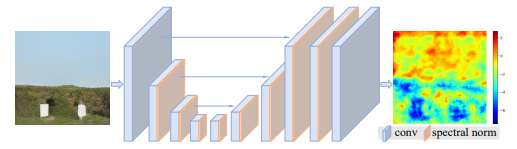
\includegraphics[scale=0.4]{figures/UNET.png}
  \caption{Architecture of the U-Net discriminator.\cite{wang2021realesrgan}}
  \label{img:UNET}
\end{figure}

The authors claim that comparisons have shown superior visual performance than prior works on various real datasets. While in this project the improved degradation model won't help much since our dataset already contains real-world degradations, the improved discriminator and better pratrained weights might yield better results compared to the previous methods.

\section{SwinIR}
\label{subsec:swinir}

CNN-based methods generally suffer from two basic
problems that stem from the basic convolution layer. First, the interactions between images and convolution kernels are content-independent. Using the same convolution kernel to restore different image regions may not be the best choice. Second, under the principle of local processing, convolution is not effective for long-range dependency modeling. As an alternative to CNN, Transformer designs a self-attention mechanism to capture global interactions between contexts and has shown promising performance in several vision problems. However, vision Transformers for image restoration usually divide the input image into patches with fixed size (e.g., 48×48) and process each patch independently. Such a strategy inevitably gives rise to two drawbacks. First, border pixels cannot utilize neighboring pixels that are out of the patch for image restoration. Second, the restored image may introduce border artifacts around each patch. While this problem can be alleviated by patch overlapping, it would introduce an extra computational burden.

More recently Swin Transformer\cite{liu2021swin}  has shown great promise as it integrates the advantages of both CNN and
Transformer. SwinIR\cite{liang2021swinir} is a Swin Transformer-based model that promises impressive performance on high-level vision tasks, such as Super Resolution and Denoising.

\begin{figure}[H]
  \centering
  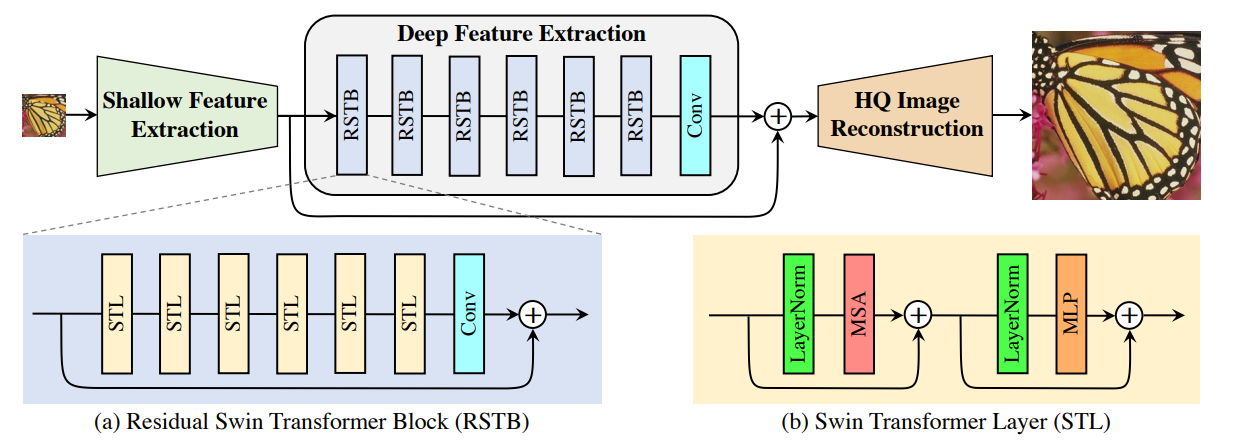
\includegraphics[scale=0.35]{figures/SwinIR.png}
  \caption{Architecture of the SwinIR model with its deep feature extraction module composed of residual Swin Transformer blocks (RSTB).\cite{liang2021swinir}}
  \label{img:swinir}
\end{figure}

\section{HAT-L}
\label{subsec:hatl}

HAT-L expands on the idea of Transformer-based methods for low-level vision tasks, such as image Super Resolution. The authors propose a novel Hybrid Attention Transformer (HAT). It combines both channel attention and window-based self-attention schemes \#TODO expand


